\section{Symmetry-Breaking Normal Form}

\subsection{Full-elastic angular sensitivities}

% Claim C2
Within the declared one-parameter cubic family, the angular and radial
coefficients were obtained from the full traction-free generalized eigenproblem,
rather than fitted from the eventual critical-point locations.  The general
Hermitian-pencil derivative in Eq.~\eqref{eq:general-frequency-sensitivity}
gave the ring sensitivity \(V(\theta)\), while the complete radial derivative in
Eq.~\eqref{eq:complete-radial-frequency-sensitivity} retained the differentiated
mode, equivalently the reduced-resolvent contribution, in \(B(\theta)\).  This
calculation is restricted to the simple tracked branch and the declared cubic
perturbation; it does not claim a coefficient formula for an arbitrary
anisotropic plate.

The resulting angular potential contained the derived pure fourfold term of
Eq.~\eqref{eq:cubic-vfour}, with signed coefficient
\(V_4=\VFour\).  Here \(V_4\) is the coefficient of the perturbation parameter,
whereas the physical fourfold frequency shift is \(\varepsilon V_4\), as fixed
by Eq.~\eqref{eq:physical-cubic-angular-shift}; the perturbation parameter is
therefore counted once.  Centered full-wave finite differences independently
recovered both \(V(\theta)\) and \(B(\theta)\).  Figure~\ref{fig:angular-sensitivity}
shows the harmonic reconstruction, the coefficient-to-shift convention, and
the finite-difference closure.  These checks make the full-elastic coefficient
closure, rather than symmetry alone, the quantitative input to the unfolding.

\begin{figure}
  \centering
  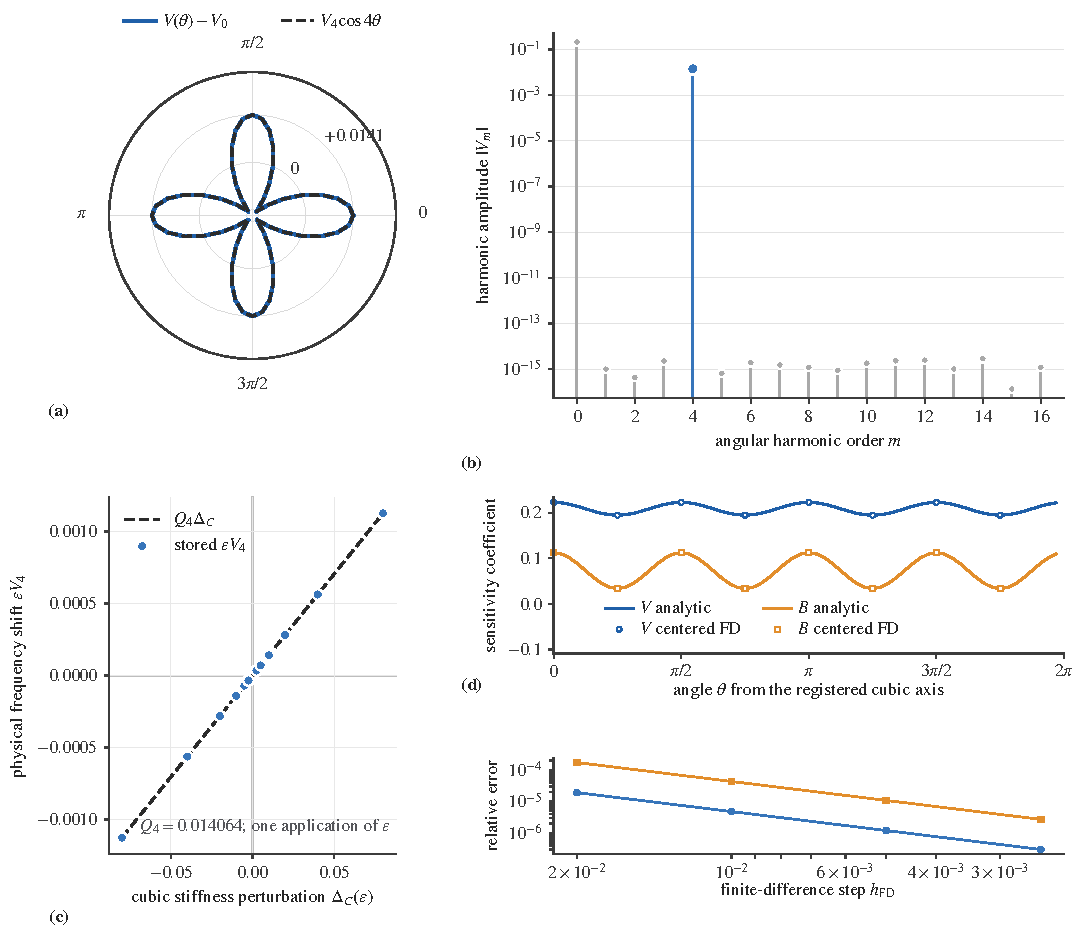
\includegraphics[width=\textwidth]{../figures/main/figure_03_angular_sensitivity.pdf}
  \caption{\FigureThreeCaption}
  \label{fig:angular-sensitivity}
\end{figure}

\subsection{Normal form and splitting theorem}

% Claim C3
Under the controlled weak-anisotropy hypotheses, eliminating the radial
stationarity equation reduced the local dispersion to an angular problem in
the declared local annulus.  Theorem~\ref{thm:anisotropic-normal-form} and
Eq.~\eqref{eq:controlled-anisotropic-normal-form} retain the radial quadratic,
the angular sensitivity, the mixed radial--angular coefficient, and a
derivative-level remainder.  The implicit radial graph in
Eq.~\eqref{eq:radial-shift} is unique in this neighborhood; substituting it
gives the reduced angular frequency of
Eq.~\eqref{eq:reduced-angular-frequency-second-order}.  These steps require a
simple separated eigenvalue and a nonzero radial curvature.

The cubic splitting theorem in Theorem~\ref{thm:cubic-morse-splitting} then
placed the critical angles and radial corrections according to
Eq.~\eqref{eq:cubic-eight-critical-points}.
For every sufficiently small nonzero \(\varepsilon\) with \(V_4\ne0\), the
theorem yields
\MorseMinimumCount{} Cartesian Morse minima and \MorseSaddleCount{} Cartesian
Morse saddles in alternating angular order.  This exact local count depends on
the derived leading harmonic and controlled remainder, not on \(C_{4v}\)
symmetry by itself and not on a global survey of every dispersion branch.

The retained isotropic radial curvature is positive.  Consequently, the sign
of the tangential curvature distinguishes the Cartesian Hessian classes: two
positive eigenvalues give a minimum, whereas one positive and one negative
eigenvalue give a saddle.  This inertia statement follows from the exact
polar-to-Cartesian Hessian in Eq.~\eqref{eq:critical-cartesian-polar-hessian}
and its Schur complement in Eq.~\eqref{eq:hessian-schur-inertia}.  A direction
with negative angular curvature is thus not a maximum.  Reversing the sign of
\(\varepsilon V_4\) exchanges the minimum and saddle angular roles while
preserving their alternating organization.  The
four-minimum/four-saddle pattern is known in anisotropic ZGV calculations
\citep{kiefer2023beating,kiefer2025skewing}; the contribution here is the
full-elastic coefficient closure together with a controlled local explanation
of why that pattern follows for this perturbation family.

\subsection{Eight resolved critical points}

% Claim C4
We restricted the full-wave search to the declared local annulus on the
tracked full-elastic branch.  The thickness discretization retained all three
displacement components.  Within this scope, the search found eight resolved roots,
comprising \MorseMinimumCount{} minima and \MorseSaddleCount{} saddles.  Every
accepted root satisfied the gradient-resolution condition associated with
Eq.~\eqref{eq:critical-point-uncertainty}, and its Cartesian Hessian eigenvalues
remained separated from their numerical discrepancy estimate.  Candidate-grid
refinement preserved the locations and alternating types.  This is a
finite-resolution local realization on one branch, not a proof of exhaustive
continuum enumeration.  In particular, the winding and grid checks cannot
exclude an unresolved opposite-index pair between candidate nodes.  Exact
four-plus-four cardinality is reserved for the sufficiently-small theorem
above, while the computed result is reported as eight refinement-stable roots.

The artifact field \texttt{morse\_index} stores the gradient, or Poincar\'e,
index rather than the number of negative Hessian eigenvalues: each resolved
minimum contributes \(+1\), each saddle contributes \(-1\), and the total is
zero.  The outer-minus-inner gradient winding agreed with this point-index sum
under Eq.~\eqref{eq:annular-index-certificate}, while both annular boundaries
remained noncritical.  Figure~\ref{fig:morse-points} displays the stored refined
coordinates, Hessian inertia, and perturbative location errors.  Point type was
assigned only when the Cartesian Hessian signs exceeded their discrepancy
estimate; it was not inferred from the appearance of interpolated contours.

\begin{figure}
  \centering
  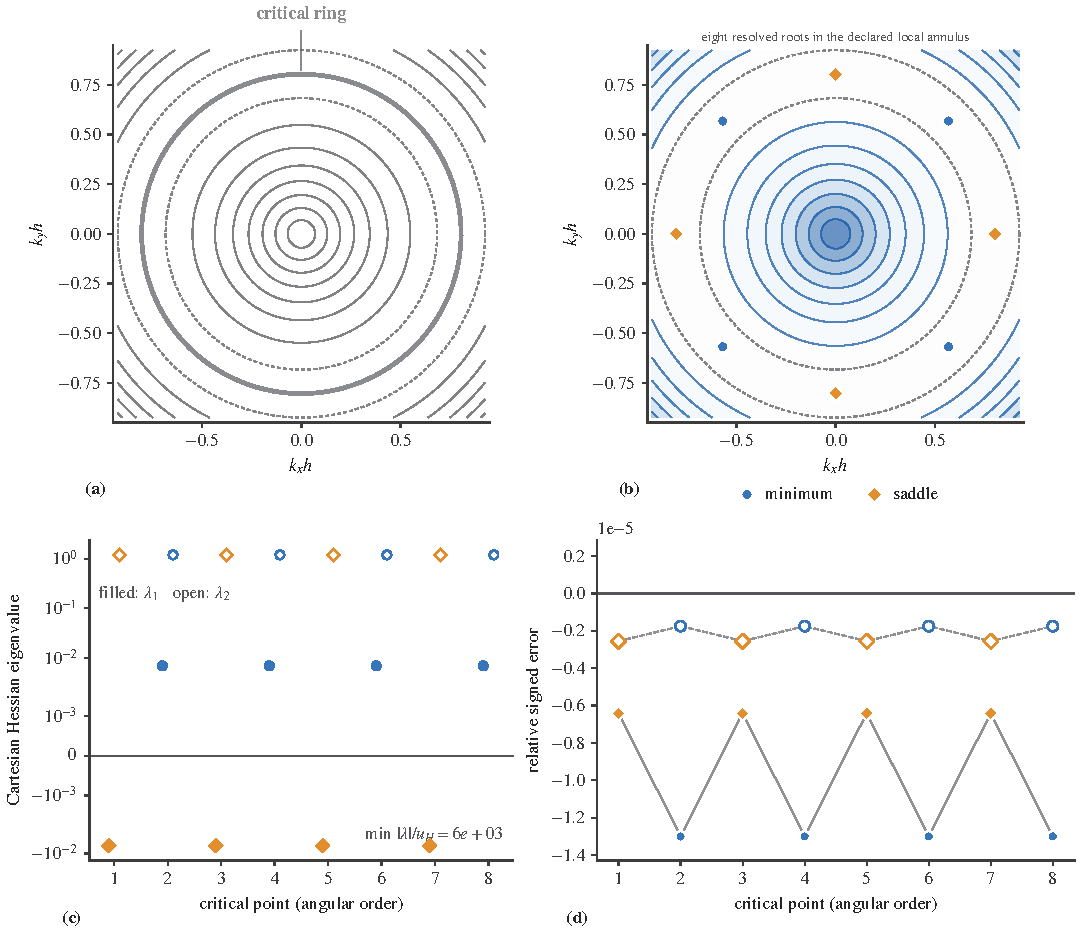
\includegraphics[width=\textwidth]{../figures/main/figure_04_morse_points.pdf}
  \caption{\FigureFourCaption}
  \label{fig:morse-points}
\end{figure}

\subsection{Scaling and sign checks}

% Claim C5
Within the predeclared weak-anisotropy sequence, compensated full-wave data
approached the radial prediction in Eq.~\eqref{eq:radial-shift}, and the
minimum--saddle critical-frequency separation followed
Eq.~\eqref{eq:cubic-minimum-saddle-separation}.  The stored log--log slope of
the separation was \SplittingSlope, consistent with first-order scaling, while
the frequency remainder slope was \RemainderSlope, consistent with a
second-order residual.  These statements are restricted to the resolved
nonzero coefficients and the declared perturbation sequence; they are not
extrapolations to a finite material anisotropy.

The compensated radial shifts and frequency remainders provide the primary
coefficient-level checks because they retain the predicted limits directly.
In particular, division by the signed perturbation approaches the full-elastic
coefficient ratio \(-B(\theta)/a\) on both angular families.
The fitted slopes are secondary summaries of those same predeclared data, not
standalone evidence or a plot-selected scaling window.  Sign reversal supplied
an independent control: changing \(\varepsilon V_4\) exchanged the angular
roles without changing the minimum and saddle counts.  Figure~\ref{fig:perturbation-scaling}
reports the complete sequence, the first- and second-order compensated
quantities, and the role-reversal check.

\begin{figure}
  \centering
  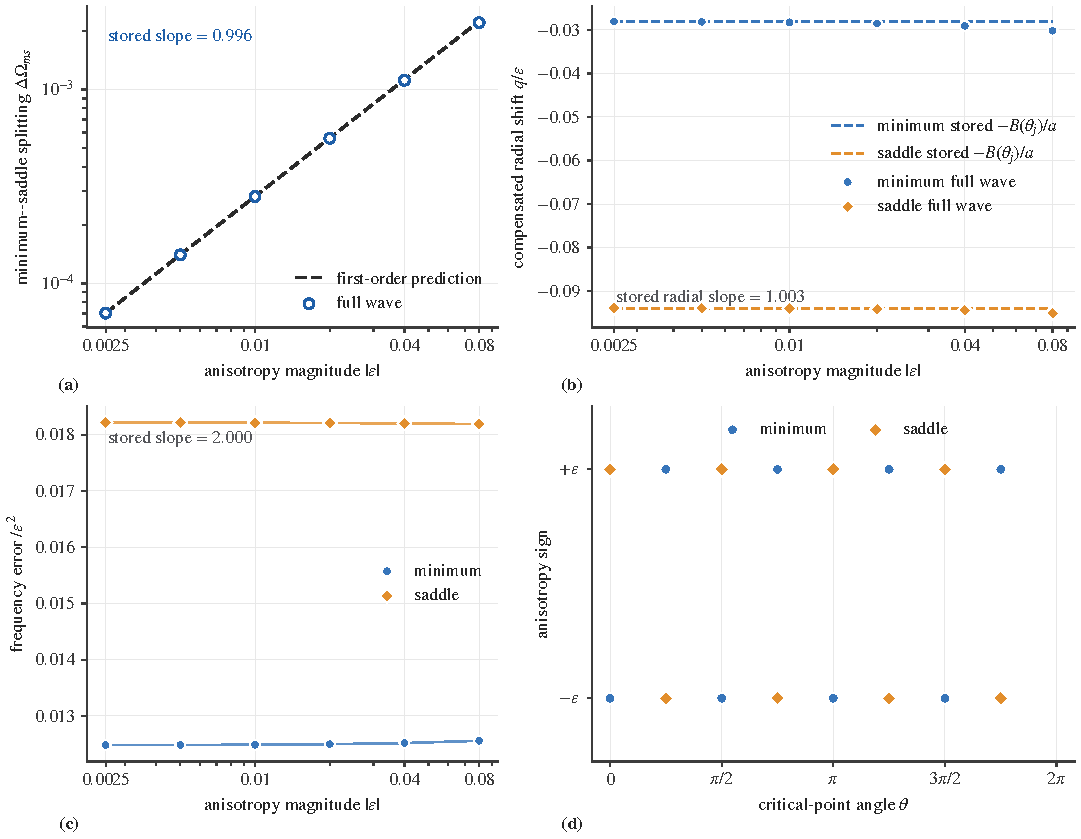
\includegraphics[width=\textwidth]{../figures/main/figure_05_perturbation_scaling.pdf}
  \caption{\FigureFiveCaption}
  \label{fig:perturbation-scaling}
\end{figure}
